\documentclass{ctexart}
\usepackage[utf8]{inputenc}
\usepackage{graphicx}
\usepackage{tikz}
\usetikzlibrary{shapes,arrows}


\title{排序算法类的实现}
\author{陈科辉 Keiver Pabula}
\date{24 November,2022}
\begin{document}
\maketitle

\section{设计思路}
首先对于heapsort和quicksort的设计我使用了与书一质的设计思路,只是我从网上拿了更全的sort头文件,只是调试时发现书顺序需要从新排序,否则会出现错误。
测试的思路首先因为要求分别比较$1\%,10\%,90\%,99\%$输入有序的情况下的排序效率,又因为数组数据不小于10000,所以我用p=10000×所要求的数据得到我应该从哪个数开始没有序。对于前面有序的从1开始到p+1是有序的,而无序的方法我就用逆序从n到p+1开始一个一个插入数组,因为在排序时逆序是最差情况的无序所以可以。然后因为要用多组数据测试,所以我用外层循环来规定,然后每次为了不同的数据所以我就用10000的k倍(k=1,2,3,4,5)来当作数组元素,对于重复实验我就重复的进行同个实验,将时间综合,再除于重复的次数得到品均消耗的时间。
\section{测试结果}
有我所设计的测试,可以得到如下的结果:
\begin{center}
  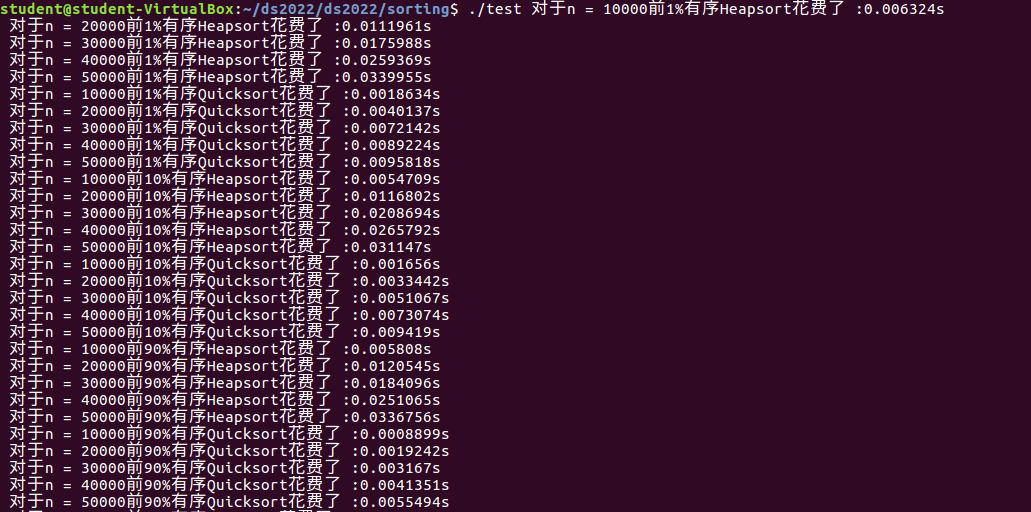
\includegraphics[scale=0.5]{ss1.png}
  \hspace{0.1in}
  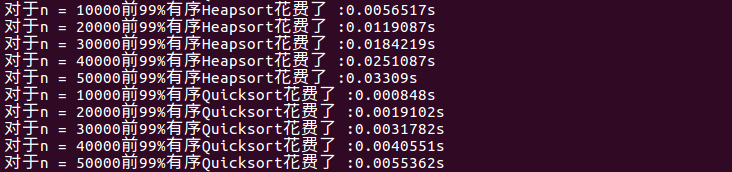
\includegraphics[scale=0.6]{ss2.png}
  \hspace{0.1in}
\end{center}
不难看出同样的n下,有序的数组越多不管是Heapsort还是Quicksort它所消耗的时间都时间都是越短的。当然当n个数组下,如果数字越小它的排序速度也会越快。最后的在n一样,有序数组的百分比也一样的情况下,Quicksort所消耗的时间远远短于HeapSort。


\end{document}
